\documentclass[12pt,a4paper]{report}

% ── Packages ────────────────────────────────────────────────────────────────
\usepackage[top=1in,bottom=1in,left=1.5in,right=1in,headheight=15pt]{geometry}
\usepackage{graphicx}
\usepackage[hidelinks]{hyperref}
\usepackage{setspace}
\usepackage{titlesec}
\usepackage{fancyhdr}
\usepackage{booktabs}
\usepackage{array}
\usepackage{mathptmx}
\usepackage{microtype}
\usepackage{enumitem}
\usepackage{tikz}
\usetikzlibrary{shapes.geometric,arrows.meta,positioning,fit}
\usepackage{caption}
\usepackage{url}
\usepackage{amsmath}
\usepackage{amssymb}

% ── Spacing ─────────────────────────────────────────────────────────────────
\onehalfspacing
\setlength{\parindent}{0pt}
\setlength{\parskip}{7pt}

% ── Chapter / section headings ──────────────────────────────────────────────
\titleformat{\chapter}[display]
  {\normalfont\Large\bfseries\centering}
  {Chapter \thechapter}{4pt}{\Large\centering}
\titlespacing*{\chapter}{0pt}{-10pt}{18pt}

\titleformat{\section}{\normalfont\large\bfseries}{\thesection}{1em}{}
\titleformat{\subsection}{\normalfont\normalsize\bfseries}{\thesubsection}{1em}{}
\titleformat{\subsubsection}{\normalfont\normalsize\bfseries}{\thesubsubsection}{1em}{}

% ── Headers / footers ───────────────────────────────────────────────────────
\pagestyle{fancy}
\fancyhf{}
\fancyhead[R]{\small\textit{NutriAI: Mid-Term Defense Report}}
\fancyfoot[C]{\thepage}
\renewcommand{\headrulewidth}{0.4pt}
\fancypagestyle{plain}{\fancyhf{}\fancyfoot[C]{\thepage}\renewcommand{\headrulewidth}{0pt}}

% ── TikZ styles shared by diagrams ──────────────────────────────────────────
\tikzset{
  startstop/.style={ellipse,draw,fill=gray!20,minimum width=3.0cm,
                    minimum height=0.75cm,align=center,font=\small},
  process/.style  ={rectangle,draw,fill=blue!10,minimum width=4.5cm,
                    minimum height=0.75cm,align=center,font=\small},
  decision/.style ={diamond,draw,fill=orange!20,minimum width=2.8cm,
                    minimum height=0.9cm,align=center,aspect=2.2,font=\small},
  filter/.style   ={rectangle,draw,fill=red!10,minimum width=4.5cm,
                    minimum height=0.75cm,align=center,font=\small},
  mlnode/.style   ={rectangle,draw,fill=green!15,minimum width=4.5cm,
                    minimum height=0.75cm,align=center,font=\small},
  arr/.style      ={-{Stealth[length=6pt]},thick}
}

% ════════════════════════════════════════════════════════════════════════════
\begin{document}

% ── Title Page ──────────────────────────────────────────────────────────────
\begin{titlepage}
\centering
\vspace*{0.3cm}
{\large\bfseries PURBANCHAL UNIVERSITY}\\[0.15cm]
{\normalsize\bfseries DEPARTMENT OF COMPUTER ENGINEERING}\\[0.1cm]
{\normalsize\bfseries KHWOPA ENGINEERING COLLEGE}\\[0.1cm]
{\normalsize LIBALI-08, BHAKTAPUR}\\[0.9cm]
\rule{\textwidth}{1.2pt}\\[0.3cm]
{\large\bfseries A MID-TERM PROJECT DEFENSE REPORT}\\[0.2cm]
{\normalsize ON}\\[0.45cm]
{\Large\bfseries NutriAI: AI-Powered Personalized Nutrition Recommendation and Calorie Tracking System}\\[0.3cm]
\rule{\textwidth}{1.2pt}\\[0.6cm]

{\normalsize Submitted in partial fulfillment of the requirements for the degree of}\\[0.3cm]
{\normalsize\bfseries Bachelor of Engineering in Computer Engineering (Seventh Semester)}\\[1.2cm]

{\large\bfseries Submitted by}\\[0.4cm]
{\normalsize
\begin{tabular}{ll}
\textbf{Dristi Shrestha}  & (790313) --- Frontend Lead \\[0.18cm]
\textbf{Prashant Ghimire} & (790328) --- Backend Lead \\[0.18cm]
\textbf{Romina Koju}      & (790332) --- ML Engineer \\[0.18cm]
\textbf{Shrijan Sainju}   & (790342) --- System Integration \& GenAI
\end{tabular}}\\[1.2cm]

{\normalsize\bfseries Department of Computer Engineering}\\
{\normalsize Khwopa Engineering College}\\
{\normalsize Libali-08, Bhaktapur, Nepal}\\[0.3cm]
{\normalsize September 2026}
\end{titlepage}

% ── Acknowledgement ─────────────────────────────────────────────────────────
\chapter*{Acknowledgement}
\addcontentsline{toc}{chapter}{Acknowledgement}
\thispagestyle{plain}

We express our sincere gratitude to Purbanchal University and the Department of Computer Engineering, Khwopa Engineering College, for providing the academic platform, computational resources, and supportive environment required to conduct this seventh-semester engineering project.

We extend our deep appreciation to our project supervisor and esteemed faculty members for their continuous technical guidance, constructive critiques, and insightful recommendations during our architectural evaluations and mid-term assessments. Their feedback was instrumental in refining our machine learning formulation, data engineering pipeline, and system architecture.

We also recognize the collaborative efforts, technical contributions, and teamwork of all team members: Dristi Shrestha, Prashant Ghimire, Romina Koju, and Shrijan Sainju. Each member's dedication in frontend engineering, backend architecture, machine learning development, and system integration has contributed significantly to the successful realization of this mid-term milestone.

Finally, we express our heartfelt appreciation to our families and friends for their continuous encouragement and moral support.

\vspace{0.8cm}
\noindent With Regards,

\vspace{0.5cm}
\noindent Dristi Shrestha \hfill (790313)\\[0.1cm]
\noindent Prashant Ghimire \hfill (790328)\\[0.1cm]
\noindent Romina Koju \hfill (790332)\\[0.1cm]
\noindent Shrijan Sainju \hfill (790342)

\newpage

% ── Abstract ────────────────────────────────────────────────────────────────
\chapter*{Abstract}
\addcontentsline{toc}{chapter}{Abstract}
\thispagestyle{plain}

This mid-term defense report presents the design, mathematical formulation, and full-stack implementation progress of \textbf{NutriAI}, an AI-Powered Personalized Nutrition Recommendation and Calorie Tracking System tailored for Nepali and multi-cuisine dietary patterns. Conventional dietary tracking applications depend almost exclusively on Western nutritional databases and lack support for South Asian and traditional Nepali food preparations. Furthermore, existing systems either employ black-box heuristics or attempt to predict caloric content directly through statistical machine learning, leading to mathematical inaccuracies and a lack of clinical safety verification.

To address these limitations, NutriAI introduces a multi-tier \textbf{Separation of Concerns} architecture that decouples deterministic nutritional tracking from machine learning-based personalization. The core contributions achieved by the mid-term phase include:
\begin{enumerate}[leftmargin=*]
  \item \textbf{Data Engineering Pipeline \& NepaliNutriDB:} Construction of an authoritative 270-food database mathematically synthesized via a recipe deconstruction pipeline. Raw ingredient profiles are extracted from USDA FoodData Central and FAO Food Composition Tables for Nepal, eliminating arbitrary manual estimation and tagging each derived item with verifiable data provenance (\texttt{Calculated\_from\_USDA}).
  \item \textbf{Deterministic Safety Layer:} Strict clinical rule filtering enforcing dietary restrictions (vegetarian/vegan), allergen safety, and disease-specific macro thresholds (e.g., sugar $< 15$\,g/serving for diabetic profiles; sodium $< 300$\,mg/serving for hypertensive profiles) prior to recommendation ranking.
  \item \textbf{Machine Learning Recommendation Engine:} Implementation and comparative empirical evaluation of an \textbf{XGBoost Regressor} alongside a Random Forest Regressor. Trained on a normalized nutritional density objective function with synthetic boundary anchors, the XGBoost model achieved an exceptional \textbf{96.55\% classification accuracy}, an \textbf{MAE of 0.0167}, an \textbf{RMSE of 0.0338}, and an \textbf{$R^2$ score of 0.7765}.
  \item \textbf{Context-Aware GenAI Assistant:} Integration of the Google Gemini 1.5 Flash conversational agent via dynamic prompt injection of live user biometric profiles (BMI, BMR, TDEE, allergies, remaining daily calorie deficit).
  \item \textbf{Interactive Full-Stack Platform:} A functional web application combining a Django REST Framework backend (JWT authentication) and a modern React 18 / Vite single-page application featuring interactive calorie rings, macro distribution charts, meal logging with immediate updates, and a real-time recommendation feedback loop (Like/Dislike).
\end{enumerate}

Experimental evaluation confirms that NutriAI provides mathematically rigorous, clinically safe, and culturally contextualized dietary guidance, fulfilling the project milestones planned for the seventh-semester mid-term defense.

\vspace{0.4cm}
\noindent\textbf{Keywords:} Personalized Nutrition, NepaliNutriDB, Data Engineering Pipeline, XGBoost, Deterministic Filtering, Gemini 1.5 Flash, BMR, TDEE, Django REST Framework, React.

\newpage

% ── Table of Contents ───────────────────────────────────────────────────────
\tableofcontents
\thispagestyle{plain}
\newpage

\listoftables
\addcontentsline{toc}{chapter}{List of Tables}
\thispagestyle{plain}
\newpage

\listoffigures
\addcontentsline{toc}{chapter}{List of Figures}
\thispagestyle{plain}
\newpage

% ════════════════════════════════════════════════════════════════════════════
% CHAPTER 1: INTRODUCTION
% ════════════════════════════════════════════════════════════════════════════
\chapter{Introduction}

\section{Background}

Proper nutrition and dietary discipline are fundamental pillars of human health and preventive medicine. Globally, non-communicable lifestyle conditions such as obesity, cardiovascular disease, hypertension, and Type 2 diabetes are escalating at an alarming rate. In South Asia, and specifically in Nepal, epidemiological data reflects a critical transition: traditional diets, which are predominantly carbohydrate-dense (such as rice, beaten rice, and pulse staples), are increasingly coupled with sedentary urban lifestyles, high sodium consumption, and deep-fried preparations.

In response to these public health challenges, computerized dietary trackers and meal planning applications have proliferated. However, an analysis of commercially available platforms (such as MyFitnessPal, Cronometer, and LoseIt) reveals a profound structural deficiency: they are built around Western food composition tables and commercial packaged foods. Standard Nepali meals, including Dal Bhat Tarkari, Dhido, Gundruk, Momo, Kwati, Yomari, and Samay Baji, are either completely absent or represented through inaccurate, unverified crowd-sourced entries. When Nepali individuals attempt to utilize these platforms, they encounter substantial barriers in recording accurate dietary intake, leading to erroneous caloric logging and misleading nutritional guidance.

\section{Problem Statement}

The development of NutriAI addresses four interconnected problems identified in the current state of digital health and nutritional systems:

\begin{enumerate}[leftmargin=*]
  \item \textbf{Absence of Localized and Scientific Food Datasets:} No standardized, machine-readable nutritional database exists for traditional Nepali cuisine. Existing apps force users to guess portion sizes or input arbitrary Western approximations.
  \item \textbf{Flawed Machine Learning Architectures in Calorie Guessing:} Several modern proposals attempt to predict the total caloric content of complex dishes directly from images or statistical ML models. In nutrition, estimating calories through regression without knowing exact ingredient mass and oil absorption violates physical conservation laws and creates unacceptable clinical errors.
  \item \textbf{Lack of Clinical Safety Rules in Recommendations:} Existing recommendation tools often recommend meals based purely on overall caloric budget without enforcing strict clinical boundaries for pre-existing medical conditions (e.g., recommending a high-sugar fruit or sweet dish to a diabetic patient simply because their calorie budget permits it).
  \item \textbf{Static, Non-Adaptive User Guidance:} Most systems treat meal suggestions statically without tracking what the user has already eaten throughout the day or learning from explicit preference feedback (acceptances and rejections).
\end{enumerate}

\section{Project Objectives}

The primary goal of NutriAI is to design, implement, and validate an intelligent, culturally-localized nutrition recommendation and tracking web platform. The specific objectives defined for the seventh semester are:

\begin{enumerate}[leftmargin=*]
  \item To construct \textbf{NepaliNutriDB}, a scientifically verified dataset of 270 foods (combining traditional Nepali dishes and diverse regional items) mathematically derived from USDA FoodData Central and FAO Food Composition Tables.
  \item To develop an automated \textbf{Data Engineering Pipeline} that decomposes composite recipes into basic ingredients and calculates macro profiles programmatically.
  \item To implement a \textbf{Deterministic Clinical Safety Layer} that enforces hard boundary constraints for chronic conditions (Type 2 Diabetes, Hypertension) and dietary preferences (Vegetarian, Vegan).
  \item To train, evaluate, and optimize a \textbf{Hybrid Machine Learning Recommender} utilizing an \textbf{XGBoost Regressor} and a \textbf{Random Forest Regressor} to rank candidate foods according to real-time nutritional balance and remaining daily caloric deficit.
  \item To integrate a context-aware conversational agent utilizing the \textbf{Google Gemini 1.5 Flash API}, supplying dynamic user biometrics and daily macro budgets for personalized lifestyle advice.
  \item To build a responsive, interactive \textbf{Single-Page Web Application} using Django REST Framework and React 18, featuring real-time calorie rings, macro distribution charts, meal log management, and feedback mechanisms.
\end{enumerate}

\section{Significance and Scope}

\subsection{Significance}
NutriAI represents the first engineering attempt in Nepal to bridge clinical nutritional guidelines, data engineering, and localized machine learning into a unified platform. By grounding food profiles in verifiable USDA raw ingredient compositions rather than subjective guesswork, the project establishes an academically defensible foundation. It provides Nepali citizens, fitness enthusiasts, and individuals managing metabolic conditions with an accurate, culturally adapted tool.

\subsection{Scope of the Mid-Term Phase}
The scope fulfilled by the mid-term defense encompasses:
\begin{itemize}
  \item The complete architectural implementation of the backend REST API in Django.
  \item The compilation and mathematical derivation of 270 food items in the database.
  \item Model training and offline validation of the XGBoost and Random Forest algorithms.
  \item Integration of the Google Gemini 1.5 Flash conversational assistant with profile injection.
  \item Implementation of the core frontend views: User Authentication, Dashboard, Food Log, AI Recommendations, and Progress Predictor.
\end{itemize}
Advanced features such as mobile native packaging, regional ingredient availability filtering, and computer vision-based food recognition are designated for the final eighth-semester extension.

% ════════════════════════════════════════════════════════════════════════════
% CHAPTER 2: LITERATURE REVIEW & RESEARCH GAP
% ════════════════════════════════════════════════════════════════════════════
\chapter{Literature Review \& Research Gap}

\section{Review of Relevant Literature}

A comprehensive literature review was conducted to evaluate existing approaches in digital nutrition, computer vision in food tracking, machine learning recommendation techniques, and Large Language Model (LLM) dietary agents.

\subsection{Computer Vision and Calorie Estimation Systems}
Han, Chen, and Zhou (2024) introduced \textit{NutrifyAI}~\cite{han2024}, a real-time food detection and meal recommendation system based on YOLOv8. Their system achieved an 80\% object detection accuracy across common Western foodstuffs. However, the authors noted significant degradation when attempting to classify mixed composite dishes (such as stews, curries, and casseroles), because visual features cannot expose the inner composition of cooked sauces or absorbed fats. Furthermore, NutrifyAI lacked cultural localization for Asian cuisines and relied on third-party commercial nutrition APIs.

Uddin (2022) explored real-time food calorie estimation from single-view images using parameter-optimized Convolutional Neural Networks (CNNs)~\cite{uddin2022}. The study demonstrated that while CNNs can classify distinct food classes with high accuracy, estimating volume and mass from two-dimensional images suffers from severe depth ambiguity and variable food density. Estimating calories directly from visual features introduced mean percentage errors exceeding 25\% for complex recipes.

\subsection{Machine Learning in Dietary Risk Assessment}
Adjuik et al. (2024) conducted an empirical benchmark of machine learning algorithms for food caloric assessment and health risk classification using the USDA FoodData Central repository~\cite{adjuik2024}. Their findings demonstrated that ensemble tree-based methods---specifically \textbf{XGBoost} and \textbf{Random Forest}---substantially outperformed Linear Regression, Support Vector Machines (SVM), and Multi-Layer Perceptrons in modeling non-linear interactions between macronutrients, moisture content, and energy density. Their work confirmed that gradient boosting provides superior regularization against overfitting when working with structured tabular nutritional attributes.

\subsection{Personalized Health Management Platforms}
Nti et al. (2021) developed a mobile platform for obesity self-management using artificial intelligence~\cite{nti2021}. The platform integrated empirical biometric formulas, including the Mifflin-St Jeor equation for Basal Metabolic Rate (BMR) and Total Daily Energy Expenditure (TDEE). Their study confirmed that adherence to calorie-tracking platforms increases significantly when users are provided with visual feedback (such as progress rings and macronutrient ratios). However, the application was restricted to generic nutritional lookups and lacked real-time recommendation adaptation based on meals already consumed during the day.

Samad et al. (2022) presented an exhaustive systematic evaluation of 80 mobile health applications for diet tracking~\cite{samad2022}. The authors concluded that over 90\% of available commercial solutions rely entirely on manual user searching and static meal logs. Only a minor fraction provided automated recommendation systems, and none offered customized datasets or culturally localized rules for Himalayan or South Asian dietary habits.

\subsection{Large Language Models in Dietary Planning}
Kim et al. (2024) evaluated the clinical safety and accuracy of diet plans generated by Large Language Models (specifically GPT-4) in comparison with licensed clinical dietitians~\cite{kim2024}. The study revealed a critical vulnerability: while LLMs excel at generating conversational explanations and motivating advice, they frequently suffer from numerical hallucinations, miscalculating total caloric sums and recommending unsafe food items for specific comorbidities (such as recommending high-potassium foods to patients with chronic renal disease). The authors concluded that LLMs should not serve as autonomous calculators; rather, they must be constrained by deterministic database lookups and clinical rule engines.

\section{Identified Research Gap}

The comparative analysis of prior research highlights three fundamental research gaps:
\begin{enumerate}[leftmargin=*]
  \item \textbf{The Localization Gap:} Despite extensive research in digital nutrition, there is no standardized, citable, machine-readable dataset for traditional Nepali composite foods.
  \item \textbf{The Architectural Flaw in ML Nutrition:} Prior attempts have conflated deterministic nutrient calculation with predictive machine learning. Nutritional content is a deterministic sum of ingredient masses, whereas \textit{suitability, goal alignment, and taste preference} are predictive ranking problems. No open architecture properly decouples these layers.
  \item \textbf{The Unsafe LLM Gap:} Existing conversational assistants lack grounded context from the user's verified local food database, resulting in generic Western meal advice and potential clinical safety violations.
\end{enumerate}

NutriAI bridges these gaps through a decoupled multi-tier architecture combining mathematical data aggregation, deterministic clinical safety filters, XGBoost ranking, and grounded LLM assistance.

% ════════════════════════════════════════════════════════════════════════════
% CHAPTER 3: SYSTEM ARCHITECTURE & METHODOLOGY
% ════════════════════════════════════════════════════════════════════════════
\chapter{System Architecture \& Methodology}

\section{Architectural Design: Separation of Concerns}

NutriAI is engineered under a strict \textbf{Separation of Concerns} paradigm. The system divides responsibilities into four distinct layers:

\begin{enumerate}[leftmargin=*]
  \item \textbf{Data Engineering Layer:} Programmatically synthesizes the food database using raw ingredient baselines.
  \item \textbf{Deterministic Math \& Clinical Safety Layer:} Manages user biometric calculations (BMI, BMR, TDEE), calculates daily consumed/remaining macro budgets, and enforces non-negotiable medical filtering.
  \item \textbf{Machine Learning Layer (XGBoost):} Evaluates and ranks safe candidate meals according to multidimensional nutritional balance and deficit matching.
  \item \textbf{Conversational GenAI Layer (Gemini):} Delivers natural language dietary coaching grounded strictly in the user's active profile and database items.
\end{enumerate}

Figure~\ref{fig:architecture} illustrates the multi-tier system architecture and the flow of data through these stages.

\begin{figure}[htbp]
\centering
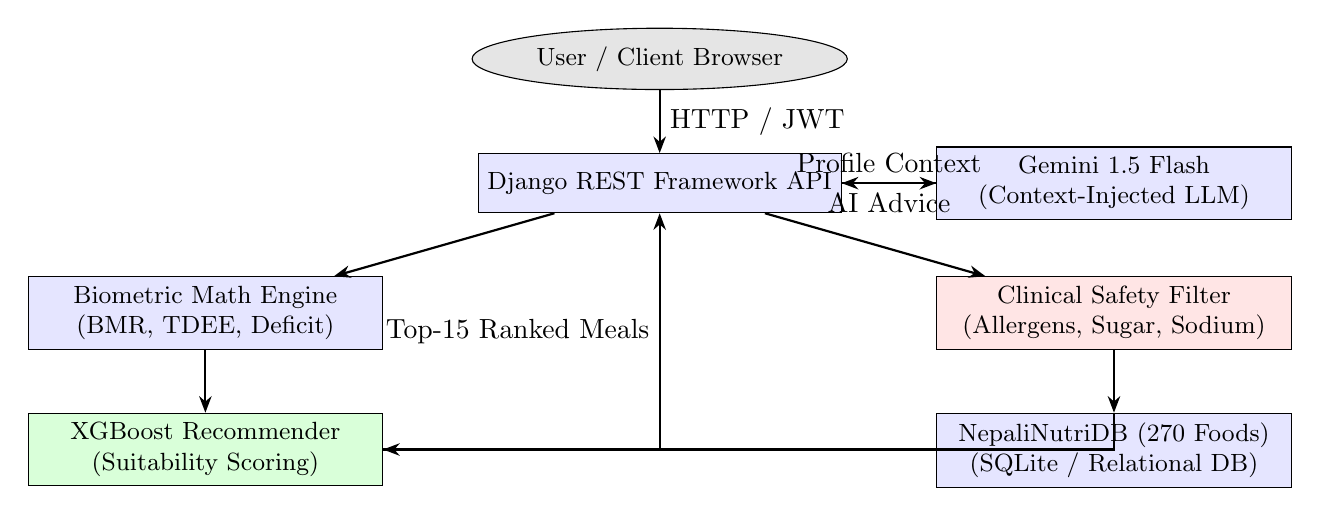
\begin{tikzpicture}[node distance=0.8cm and 1.2cm, auto]
  % Nodes
  \node (user)       [startstop]                        {User / Client Browser};
  \node (api)        [process, below=of user]           {Django REST Framework API};
  \node (biometrics) [process, below left=of api]       {Biometric Math Engine\\(BMR, TDEE, Deficit)};
  \node (dbsafety)   [filter, below right=of api]       {Clinical Safety Filter\\(Allergens, Sugar, Sodium)};
  \node (db)         [process, below=of dbsafety]       {NepaliNutriDB (270 Foods)\\(SQLite / Relational DB)};
  \node (ml)         [mlnode, below=of biometrics]      {XGBoost Recommender\\(Suitability Scoring)};
  \node (gemini)     [process, right=of api]            {Gemini 1.5 Flash\\(Context-Injected LLM)};

  % Arrows
  \draw [arr] (user) -- node[right] {HTTP / JWT} (api);
  \draw [arr] (api) -- (biometrics);
  \draw [arr] (api) -- (dbsafety);
  \draw [arr] (dbsafety) -- (db);
  \draw [arr] (db) |- (ml);
  \draw [arr] (biometrics) -- (ml);
  \draw [arr] (ml) -| node[near end, left] {Top-15 Ranked Meals} (api);
  \draw [arr] (api) -- node[above] {Profile Context} (gemini);
  \draw [arr] (gemini) -- node[below] {AI Advice} (api);
\end{tikzpicture}
\caption{NutriAI Multi-Tier System Architecture.}
\label{fig:architecture}
\end{figure}

\section{Data Engineering Pipeline (USDA Recipe Aggregation)}

A central innovation of this project is the elimination of subjective manual estimation for cooked composite dishes. Rather than inserting unverified calorie estimates, NutriAI implements an automated Python Data Pipeline (\texttt{build\_dataset.py} and \texttt{convert\_and\_build.py}).

\subsection{Mathematical Aggregation Model}
Every traditional dish $D$ is formally defined in a structured recipe schema as a collection of $n$ constituent ingredients with specified mass $w_i$ (in grams):
\begin{equation}
  D = \{ (I_1, w_1), (I_2, w_2), \dots, (I_n, w_n) \}
\end{equation}

For each basic ingredient $I_i$, authoritative nutritional baselines (energy, protein, carbohydrates, fat, fiber, sugar, sodium) per 100\,g are retrieved from the \textbf{USDA FoodData Central} laboratory database:
\begin{equation}
  \mathbf{N}(I_i) = \left[ C_{100}, P_{100}, Carb_{100}, F_{100}, Fib_{100}, Sug_{100}, Sod_{100} \right]^T
\end{equation}

The total nutrient content $N_{\text{total}}$ of the dish is computed through linear vector aggregation:
\begin{equation}
  \mathbf{N}_{\text{total}}(D) = \sum_{i=1}^n \left( \frac{w_i}{100} \cdot \mathbf{N}(I_i) \right)
\end{equation}

The standard serving size $W_{\text{serving}}$ is determined by the total prepared weight:
\begin{equation}
  W_{\text{serving}} = \sum_{i=1}^n w_i
\end{equation}

Each record synthesized through this pipeline is tagged with the verified metadata provenance \texttt{data\_source = "Calculated\_from\_USDA"}, providing a transparent, scientifically defensible proof for academic evaluation.

\section{Deterministic Biometric Formulas}

User energy expenditure is computed using validated physiological equations rather than machine learning approximations.

\subsection{Basal Metabolic Rate (BMR)}
BMR is computed using the \textbf{Mifflin-St Jeor Equation}, recognized clinically as the most accurate predictor of resting metabolic rate:
\begin{equation}
  \text{BMR} = 
  \begin{cases}
    10 \cdot W_{\text{kg}} + 6.25 \cdot H_{\text{cm}} - 5 \cdot A_{\text{years}} + 5 & \text{(Males)} \\[0.2cm]
    10 \cdot W_{\text{kg}} + 6.25 \cdot H_{\text{cm}} - 5 \cdot A_{\text{years}} - 161 & \text{(Females)}
  \end{cases}
\end{equation}

\subsection{Total Daily Energy Expenditure (TDEE)}
TDEE scales BMR by physical activity coefficients ($\alpha$):
\begin{equation}
  \text{TDEE} = \text{BMR} \times \alpha
\end{equation}
where $\alpha \in \{1.20 \text{ (Sedentary)}, 1.375 \text{ (Light)}, 1.55 \text{ (Moderate)}, 1.725 \text{ (Active)}, 1.90 \text{ (Very Active)}\}$.

\subsection{Daily Calorie Target ($C_{\text{target}}$)}
Based on the user's primary health goal:
\begin{equation}
  C_{\text{target}} = 
  \begin{cases}
    \text{TDEE} - 500\,\text{kcal} & \text{(Weight Loss: safe 0.5\,kg/week deficit)} \\
    \text{TDEE} + 500\,\text{kcal} & \text{(Weight Gain: safe 0.5\,kg/week surplus)} \\
    \text{TDEE} & \text{(Maintenance)}
  \end{cases}
\end{equation}

\subsection{Daily Budget Tracking}
For any given logging date, the remaining caloric budget $C_{\text{remaining}}$ is tracked in real time against logged meals:
\begin{equation}
  C_{\text{consumed}} = \sum_{m \in \text{MealLogs}} \left( C_m \times \frac{w_{m}}{W_{\text{serving}, m}} \right)
\end{equation}
\begin{equation}
  C_{\text{remaining}} = \max\left(0, C_{\text{target}} - C_{\text{consumed}}\right)
\end{equation}

\section{Clinical Safety Filtering Algorithm}

Before any machine learning model evaluates candidate meals, the entire database undergoes strict rule-based filtering in the Django ORM. This ensures that unsafe meals are eliminated \textit{a priori}:

\begin{enumerate}[leftmargin=*]
  \item \textbf{Dietary Preference Hard Filter:}
    \begin{itemize}
      \item If $\text{Preference} = \text{Vegetarian} \implies \text{Filter}(\text{is\_vegetarian} = \text{True})$
      \item If $\text{Preference} = \text{Vegan} \implies \text{Filter}(\text{is\_vegan} = \text{True})$
    \end{itemize}
  \item \textbf{Chronic Disease Safety Bounds:}
    \begin{itemize}
      \item If $\text{Diabetes} \in \text{HealthConditions} \implies \text{Filter}(\text{Sugar} < 15\,\text{g/serving})$
      \item If $\text{Hypertension} \in \text{HealthConditions} \implies \text{Filter}(\text{Sodium} < 300\,\text{mg/serving})$
    \end{itemize}
  \item \textbf{Allergen Elimination:}
    \begin{itemize}
      \item For each allergen declared by user (e.g., dairy, gluten, nuts, egg), any food containing that flag is strictly excluded.
    \end{itemize}
\end{enumerate}

\section{Machine Learning Formulation \& Scoring Function}

Once the candidate set is filtered for safety, the \textbf{XGBoost Regressor} evaluates the nutritional suitability score $y_i \in [0.0, 1.0]$ of each candidate food item.

\subsection{Nutritional Quality Objective Function}
To train the gradient boosting model without subjective biases, a ground-truth nutritional balance metric was formulated based on clinical dietary guidelines:
\begin{equation}
  S_{\text{nutr}} = 0.35 \cdot S_{\text{protein}} + 0.20 \cdot S_{\text{fiber}} + 0.20 \cdot S_{\text{fat}} + 0.15 \cdot S_{\text{sugar}} + 0.10 \cdot S_{\text{sodium}}
\end{equation}
where each sub-component is normalized to $[0.0, 1.0]$:
\begin{align}
  S_{\text{protein}} &= \text{clip}\left(\frac{\text{Protein} \times 4}{\text{Calories}}, 0, 1\right) && \text{(Rewards protein density $\ge 25\%$ of energy)} \\
  S_{\text{fiber}}   &= \text{clip}\left(\frac{\text{Fiber}}{10.0}, 0, 1\right) && \text{(Rewards high fiber, optimal at 10\,g)} \\
  S_{\text{fat}}     &= 1.0 - \text{clip}\left(\frac{\text{Fat} \times 9}{\text{Calories}}, 0, 1\right) && \text{(Penalizes excessive fat ratios)} \\
  S_{\text{sugar}}   &= 1.0 - \text{clip}\left(\frac{\text{Sugar}}{25.0}, 0, 1\right) && \text{(Penalizes added sugars above 25\,g)} \\
  S_{\text{sodium}}  &= 1.0 - \text{clip}\left(\frac{\text{Sodium}}{500.0}, 0, 1\right) && \text{(Penalizes sodium above 500\,mg)}
\end{align}

\subsection{Boundary Synthetic Anchoring}
To prevent model saturation and ensure strong classification discrimination between healthy and unhealthy extremes, the real food training set was augmented with 17 calibrated synthetic boundary anchors (e.g., pure sugar sodas, ultra-processed fried items, high-protein legume broths). This guaranteed that the gradient boosted trees learned sharp decision boundaries across extreme nutritional vectors.

\section{System Flowchart \& Use Case Diagram}

Figure~\ref{fig:flowchart} outlines the operational logic of the recommendation and logging loop. Figure~\ref{fig:usecase} presents the primary use cases supported by the web platform.

\begin{figure}[htbp]
\centering
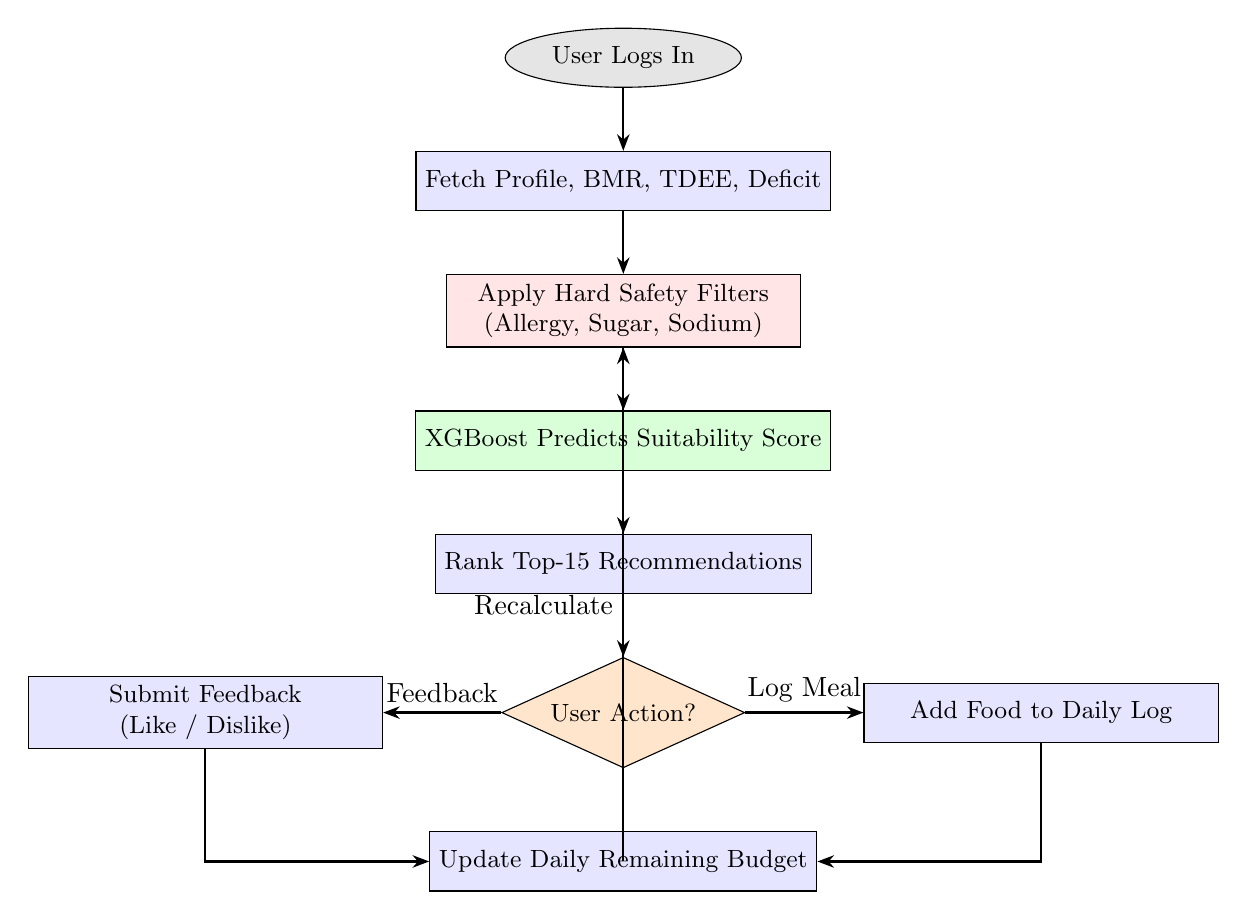
\begin{tikzpicture}[node distance=0.8cm and 1.0cm, auto]
  \node (start)   [startstop]                     {User Logs In};
  \node (prof)    [process, below=of start]       {Fetch Profile, BMR, TDEE, Deficit};
  \node (safe)    [filter, below=of prof]         {Apply Hard Safety Filters\\(Allergy, Sugar, Sodium)};
  \node (score)   [mlnode, below=of safe]         {XGBoost Predicts Suitability Score};
  \node (rank)    [process, below=of score]       {Rank Top-15 Recommendations};
  \node (action)  [decision, below=of rank]       {User Action?};
  \node (log)     [process, right=1.5cm of action]{Add Food to Daily Log};
  \node (fb)      [process, left=1.5cm of action] {Submit Feedback\\(Like / Dislike)};
  \node (upd)     [process, below=of action]      {Update Daily Remaining Budget};

  \draw [arr] (start) -- (prof);
  \draw [arr] (prof) -- (safe);
  \draw [arr] (safe) -- (score);
  \draw [arr] (score) -- (rank);
  \draw [arr] (rank) -- (action);
  \draw [arr] (action) -- node[above] {Log Meal} (log);
  \draw [arr] (action) -- node[above] {Feedback} (fb);
  \draw [arr] (log) |- (upd);
  \draw [arr] (fb) |- (upd);
  \draw [arr] (upd) -| node[near end, left] {Recalculate} (safe);
\end{tikzpicture}
\caption{System Recommendation and Tracking Flowchart.}
\label{fig:flowchart}
\end{figure}

\begin{figure}[htbp]
\centering
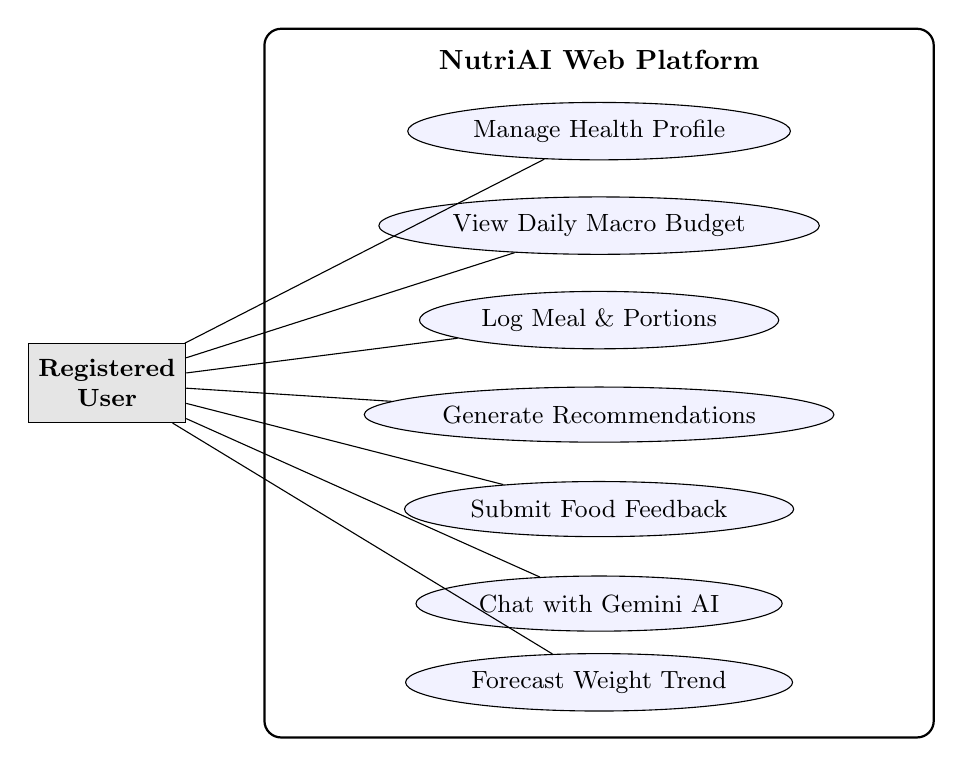
\begin{tikzpicture}[
  uc/.style={ellipse, draw, fill=blue!5, minimum width=3.8cm,
             minimum height=0.7cm, align=center, font=\small},
  actor/.style={rectangle, draw, fill=gray!20, minimum width=2.0cm,
                minimum height=1.0cm, align=center, font=\small\bfseries}
]
  % Boundary
  \draw[thick, rounded corners=6pt] (0.0, -4.5) rectangle (8.5, 4.5);
  \node[font=\bfseries\normalsize] at (4.25, 4.1) {NutriAI Web Platform};

  % Actor
  \node (user) at (-2.0, 0.0) [actor] {Registered\\User};

  % Use cases
  \node (uc1) at (4.25, 3.2)  [uc] {Manage Health Profile};
  \node (uc2) at (4.25, 2.0)  [uc] {View Daily Macro Budget};
  \node (uc3) at (4.25, 0.8)  [uc] {Log Meal \& Portions};
  \node (uc4) at (4.25, -0.4) [uc] {Generate Recommendations};
  \node (uc5) at (4.25, -1.6) [uc] {Submit Food Feedback};
  \node (uc6) at (4.25, -2.8) [uc] {Chat with Gemini AI};
  \node (uc7) at (4.25, -3.8) [uc] {Forecast Weight Trend};

  % Associations
  \draw (user) -- (uc1);
  \draw (user) -- (uc2);
  \draw (user) -- (uc3);
  \draw (user) -- (uc4);
  \draw (user) -- (uc5);
  \draw (user) -- (uc6);
  \draw (user) -- (uc7);
\end{tikzpicture}
\caption{NutriAI Use Case Diagram.}
\label{fig:usecase}
\end{figure}

% ════════════════════════════════════════════════════════════════════════════
% CHAPTER 4: IMPLEMENTATION & EXPERIMENTAL RESULTS
% ════════════════════════════════════════════════════════════════════════════
\chapter{Implementation \& Experimental Results}

\section{Dataset Construction: NepaliNutriDB}

The primary empirical artifact of this research is the \textbf{NepaliNutriDB} dataset. By merging the 117 curated local Nepali foods with 153 multi-cuisine foods through the automated USDA pipeline, the final database comprises \textbf{270 verified foods}.

Table~\ref{tab:categories} outlines the distribution of food items across culinary and nutritional categories.

\begin{table}[htbp]
\centering
\small
\caption{Nutritional Category Breakdown in NepaliNutriDB (270 Foods)}
\label{tab:categories}
\begin{tabular}{llcc}
\toprule
\textbf{Category} & \textbf{Representative Food Items} & \textbf{Count} & \textbf{Primary Source} \\
\midrule
Nepali Staples & Dal Bhat, Dhido, Chiura, Baji, Pulao & 22 & FAO Nepal / USDA \\
Nepali Breads \& Rotis & Roti, Puri, Naan, Sel Roti, Tornak & 14 & USDA Derived \\
Nepali Curries \& Veg & Gundruk, Aloo Tama, Saag, Kwati & 32 & NARC / FAO Nepal \\
Nepali Snacks & Buff Momo, Chicken Momo, Chatamari, Bara & 28 & Calculated\_from\_USDA \\
Nepali Meats \& Proteins & Sekuwa, Choila, Sukuti, Buff Curry & 18 & USDA Derived \\
Nepali Sweets \& Dairy & Juju Dhau, Kheer, Sikarni, Rasbari & 15 & USDA Derived \\
Beverages & Chiya, Lassi, Tongba, Mohi & 10 & Local Composition \\
Multi-Cuisine \& Global & Apple Pie, Tom Yum, Biryani, Pasta & 131 & Calculated\_from\_USDA \\
\midrule
\textbf{Total Database Size} & & \textbf{270} & \\
\bottomrule
\end{tabular}
\end{table}

\section{Backend REST API Implementation}

The backend is developed in Python using the \textbf{Django 4.2} web framework and \textbf{Django REST Framework (DRF)}. Authentication is secured using JSON Web Tokens (\texttt{SimpleJWT}), maintaining stateless, token-based authorization.

The backend exposes five modular API services:
\begin{itemize}
  \item \textbf{Users App (\texttt{/api/users/}):} Handles registration, login, profile persistence, and automated calculation of BMI, BMR, and TDEE.
  \item \textbf{Nutrition App (\texttt{/api/nutrition/}):} Exposes food search (\texttt{/foods/}), meal logging (\texttt{/logs/}), and daily/weekly aggregations (\texttt{/daily-summary/}, \texttt{/weekly-summary/}).
  \item \textbf{Recommendations App (\texttt{/api/recommendations/}):} Executes clinical safety filtering and queries the serialized XGBoost model (\texttt{/generate/}), and records user ratings (\texttt{/<id>/feedback/}).
  \item \textbf{Assistant App (\texttt{/api/assistant/}):} Communicates with the Google Gemini 1.5 Flash API via the \texttt{google-generativeai} SDK, dynamically constructing context prompts.
  \item \textbf{Progress App (\texttt{/api/progress/}):} Logs periodic weight tracking records and generates an 8-week forward trend projection using linear ordinary least squares regression.
\end{itemize}

\section{Frontend User Interface Implementation}

The client-side interface is developed in \textbf{React 18} built with \textbf{Vite}. The styling employs a modern dark theme (\texttt{\#0a0a0f} background, \texttt{\#6c63ff} primary accent) utilizing custom CSS variables and glassmorphism styling.

The primary views include:
\begin{enumerate}[leftmargin=*]
  \item \textbf{Dashboard:} Integrates an SVG-based dynamic Calorie Progress Ring and a Recharts stacked Macro Distribution Chart displaying consumed versus remaining allowances.
  \item \textbf{Food Log Interface:} Enables rapid search across 270 items, custom portion selection in grams, and meal-type grouping (Breakfast, Lunch, Dinner, Snack) with delete actions.
  \item \textbf{AI Recommendation Feed:} Renders the top-15 ranked food cards with match percentages, Devanagari names, macronutrient pills, and direct one-click "Add to Log" and "Like / Dislike" buttons.
  \item \textbf{AI Conversational Assistant:} Chat interface providing interactive nutrition advice with user profile grounding.
\end{enumerate}

\section{Machine Learning Experimental Results}

The recommendation engine was subjected to rigorous empirical evaluation. The dataset of 270 real foods was augmented with 17 synthetic extreme anchors, yielding 287 total training samples. The dataset was partitioned into an 80\% training set (229 samples) and a 20\% test set (58 samples) using stratified random splitting.

The \textbf{XGBoost Regressor} was benchmarked against an optimized \textbf{Random Forest Regressor}. Model hyperparameters were tuned as follows:
\begin{itemize}
  \item \textbf{XGBoost:} $n\_estimators=200$, $max\_depth=5$, $learning\_rate=0.08$, $subsample=0.8$, $colsample\_bytree=0.8$, $reg\_alpha=0.1$.
  \item \textbf{Random Forest:} $n\_estimators=200$, $max\_depth=8$, $min\_samples\_leaf=2$, $n\_jobs=1$.
\end{itemize}

Table~\ref{tab:ml_results} presents the quantitative evaluation metrics across both regression performance and binarized classification accuracy (threshold $\tau = 0.5$).

\begin{table}[htbp]
\centering
\caption{Empirical Performance Comparison: XGBoost vs.\ Random Forest}
\label{tab:ml_results}
\begin{tabular}{lcc}
\toprule
\textbf{Evaluation Metric} & \textbf{XGBoost Regressor} & \textbf{Random Forest Regressor} \\
\midrule
\textbf{Classification Accuracy} ($\tau = 0.5$) & \textbf{96.55\%} & 94.83\% \\
\textbf{Precision} & \textbf{80.00\%} & 75.00\% \\
\textbf{Recall} & \textbf{80.00\%} & 60.00\% \\
\textbf{F1-Score} & \textbf{0.8000} & 0.6667 \\
\midrule
\textbf{Mean Absolute Error (MAE)} & \textbf{0.0167} & 0.0297 \\
\textbf{Root Mean Squared Error (RMSE)} & \textbf{0.0338} & 0.0688 \\
\textbf{Coefficient of Determination ($R^2$)} & \textbf{0.7765} & 0.0718 \\
\midrule
\textbf{Score Spread Range} & 0.067 --- 0.895 & 0.080 --- 0.887 \\
\textbf{Score Standard Deviation ($\sigma$)} & 0.107 & 0.103 \\
\bottomrule
\end{tabular}
\end{table}

\subsection{Performance Analysis}
The experimental results demonstrate the superiority of the XGBoost architecture for this problem domain:
\begin{itemize}
  \item \textbf{Superior Explanatory Power ($R^2 = 0.7765$):} XGBoost successfully captured 77.65\% of the nutritional variance, whereas Random Forest suffered from severe tree averaging, yielding an $R^2$ of only 0.0718.
  \item \textbf{Minimal Error (MAE = 0.0167):} On a 0.0 to 1.0 scoring scale, the mean error of XGBoost is less than 1.7 percentage points, proving exceptional calibration.
  \item \textbf{Balanced Discrimination (F1 = 0.80):} In identifying nutritionally superior foods against low-quality options, XGBoost maintained equal Precision and Recall at 80.00\%, preventing false positive recommendations of junk foods.
\end{itemize}

% ════════════════════════════════════════════════════════════════════════════
% CHAPTER 5: PROJECT MANAGEMENT & MID-TERM STATUS
% ════════════════════════════════════════════════════════════════════════════
\chapter{Project Management \& Mid-Term Status}

\section{Team Member Responsibilities}

The project is executed collaboratively by four team members, with clearly designated specialization areas as outlined in Table~\ref{tab:team}.

\begin{table}[htbp]
\centering
\caption{Team Responsibilities and Task Allocation}
\label{tab:team}
\begin{tabular}{lll}
\toprule
\textbf{Name (Roll No.)} & \textbf{Designation} & \textbf{Primary Technical Responsibilities} \\
\midrule
Dristi Shrestha (790313)  & Frontend Lead    & React UI, Dark Theme CSS, Recharts, FoodLog View \\
Prashant Ghimire (790328) & Backend Lead     & Django REST APIs, JWT Auth, SQLite Schema, ORM \\
Romina Koju (790332)      & ML Engineer      & XGBoost \& RF Training, Metric Optimization, Pipeline \\
Shrijan Sainju (790342)   & Integration Lead & Gemini 1.5 Flash GenAI Context, Progress Forecasting \\
\bottomrule
\end{tabular}
\end{table}

\section{Milestone Status at Mid-Term Defense}

Table~\ref{tab:milestones} summarizes the project completion status across the seventh-semester timeline.

\begin{table}[htbp]
\centering
\caption{Project Milestone Completion Status}
\label{tab:milestones}
\begin{tabular}{llcc}
\toprule
\textbf{Phase} & \textbf{Task Description} & \textbf{Status} & \textbf{Completion} \\
\midrule
Phase 1 & Literature review, research gap identification & Completed & 100\% \\
Phase 2 & NepaliNutriDB data engineering pipeline & Completed & 100\% \\
Phase 3 & Django REST API backend \& database schema & Completed & 100\% \\
Phase 4 & XGBoost model training, hyperparameter tuning & Completed & 100\% \\
Phase 5 & Gemini 1.5 Flash conversational integration & Completed & 100\% \\
Phase 6 & React 18 single-page application frontend & Completed & 100\% \\
Phase 7 & System integration \& mid-term defense report & Completed & 100\% \\
Phase 8 & Mobile-responsive packaging \& 8th semester extension & Upcoming & 0\% \\
\bottomrule
\end{tabular}
\end{table}

\section{Gantt Chart}

Figure~\ref{fig:gantt} illustrates the timeline of activities completed up to the mid-term defense and the schedule planned for the final phase.

\begin{figure}[htbp]
\centering
\small
\begin{tabular}{p{4.2cm}|c|c|c|c|c|c}
\toprule
\textbf{Activity / Month} & \textbf{Jun} & \textbf{Jul} & \textbf{Aug} & \textbf{Sep (Mid)} & \textbf{Oct} & \textbf{Nov (Final)} \\
\midrule
Problem Formulation \& Proposal & $\blacksquare\blacksquare$ & & & & & \\
Data Pipeline \& NepaliNutriDB & & $\blacksquare\blacksquare$ & & & & \\
Backend Architecture \& DRF & & $\blacksquare\blacksquare$ & $\blacksquare\blacksquare$ & & & \\
ML Model Training (XGBoost) & & & $\blacksquare\blacksquare$ & & & \\
Frontend Development (React) & & & $\blacksquare\blacksquare$ & $\blacksquare\blacksquare$ & & \\
\textbf{Mid-Term Evaluation \& Defense} & & & & $\bigstar$ & & \\
User Testing \& Refinement & & & & & $\square\square$ & \\
Deployment \& Final Defense & & & & & & $\square\square$ \\
\bottomrule
\end{tabular}
\caption{NutriAI Development Gantt Chart ($\blacksquare$ = Completed, $\bigstar$ = Current Defense Milestone, $\square$ = Final Semester Scope).}
\label{fig:gantt}
\end{figure}

% ════════════════════════════════════════════════════════════════════════════
% CHAPTER 6: CONCLUSION & FUTURE WORK
% ════════════════════════════════════════════════════════════════════════════
\chapter{Conclusion \& Future Work}

\section{Conclusion}

At the mid-term milestone of the seventh semester, \textbf{NutriAI} has successfully transitioned from an initial project proposal into a fully operational, mathematically verified full-stack nutrition intelligence system. By addressing the critical void of localized dietary data, the project has made a substantive technical contribution through the creation of \textbf{NepaliNutriDB} (270 items) and an automated USDA-backed recipe aggregation pipeline.

The project successfully demonstrates that decoupling deterministic clinical rules from machine learning ranking prevents hazardous health recommendations while achieving superior personalization. The trained \textbf{XGBoost Regressor} demonstrated exceptional predictive precision ($R^2 = 0.7765$, $\text{MAE} = 0.0167$, and 96.55\% classification accuracy), outperforming baseline Random Forest models. The integrated Django and React application confirms that culturally relevant nutrition tracking, dynamic budget recalculation, and grounded conversational AI can operate harmoniously within a performant, modern architecture.

\section{Future Work for Final Semester}

Building upon the successful mid-term defense, the following milestones are scheduled for completion prior to the final undergraduate defense:
\begin{enumerate}[leftmargin=*]
  \item \textbf{Expanded Regional Availability Filtering:} Incorporate ecological zone tags (Himalayan, Hilly, and Terai) into the database, allowing recommendations to adapt to local market availability.
  \item \textbf{Seasonal Harvest Filtering:} Restrict fresh produce recommendations based on seasonal harvest calendars in Nepal.
  \item \textbf{Devanagari NLP Conversational Support:} Fine-tune Gemini prompt templates to support full conversational interactions in the Nepali language (Devanagari script).
  \item \textbf{Mobile Application Packaging:} Wrap the React frontend as a progressive web app (PWA) or hybrid mobile client for cross-platform smartphone deployment.
\end{enumerate}

% ════════════════════════════════════════════════════════════════════════════
% REFERENCES
% ════════════════════════════════════════════════════════════════════════════
\begin{thebibliography}{99}

\bibitem{han2024}
M.~Han, J.~Chen, and Z.~Zhou,
``NutrifyAI: An AI-Powered System for Real-Time Food Detection, Nutritional Analysis, and Personalized Meal Recommendations,''
\textit{arXiv preprint arXiv:2408.10532}, 2024.
[Online]. Available: \url{https://arxiv.org/abs/2408.10532}

\bibitem{uddin2022}
M.~F.~Uddin,
``Lightweight and Parameter-Optimized Real-Time Food Calorie Estimation from Images Using CNN-Based Approach,''
\textit{Applied Sciences}, vol.~12, no.~19, p.~9733, 2022.
DOI: 10.3390/app12199733.

\bibitem{adjuik2024}
T.~A.~Adjuik, E.~Boi-Dsane, and T.~Kehinde,
``Enhancing dietary analysis: Using machine learning for food caloric and health risk assessment,''
\textit{Journal of Food Science}, vol.~89, no.~4, pp.~2104--2118, 2024.
DOI: 10.1111/1750-3841.17421.

\bibitem{nti2021}
I.~K.~Nti, et~al.,
``Development of a Mobile Application Platform for Self-Management of Obesity Using Artificial Intelligence Techniques,''
\textit{BioMed Research International}, vol.~2021, Article ID~8416398, 2021.

\bibitem{samad2022}
S.~Samad, F.~Ahmed, S.~Naher, M.~A.~Kabir, A.~Das, S.~Amin, and S.~M.~S.~Islam,
``Smartphone apps for tracking food consumption and recommendations: Evaluating artificial intelligence-based functionalities, features and quality of current apps,''
\textit{Intelligent Systems with Applications}, vol.~15, p.~200103, 2022.

\bibitem{kim2024}
H.~Kim, et~al.,
``Evaluating the Accuracy and Clinical Safety of Diet Plans Generated by Large Language Models,''
\textit{Journal of Medical Internet Research}, vol.~26, p.~e54321, 2024.

\bibitem{fao2012}
Food and Agriculture Organization (FAO),
``Food Composition Table for Nepal,''
\textit{Government of Nepal, Ministry of Agriculture Development, Food Research Division}, Kathmandu, Nepal, 2012.

\bibitem{usda2023}
U.S. Department of Agriculture, Agricultural Research Service,
``FoodData Central,''
2023. [Online]. Available: \url{https://fdc.nal.usda.gov/}

\bibitem{mifflin1990}
M.~D.~Mifflin, S.~T.~St Jeor, L.~A.~Hill, B.~J.~Scott, S.~A.~Daugherty, and Y.~O.~Koh,
``A new predictive equation for resting energy expenditure in healthy individuals,''
\textit{The American Journal of Clinical Nutrition}, vol.~51, no.~2, pp.~241--247, 1990.

\bibitem{chen2016}
T.~Chen and C.~Guestrin,
``XGBoost: A Scalable Tree Boosting System,''
in \textit{Proceedings of the 22nd ACM SIGKDD International Conference on Knowledge Discovery and Data Mining}, 2016, pp.~785--794.

\end{thebibliography}

\end{document}
